\documentclass [a4paper,11pt]{article}
\usepackage{amssymb}
\usepackage{amsthm}
\usepackage[intlimits]{amsmath}
\usepackage[polish]{babel}
\usepackage[utf8]{inputenc}
\usepackage[T1]{fontenc}
\frenchspacing
\usepackage{indentfirst}
\usepackage{graphicx}
\usepackage{subfig}
\usepackage{mathptmx}
\usepackage{geometry}
\usepackage{wrapfig}
\usepackage{enumitem}
\usepackage{tabularx}

\title{Moduł Younga}
\author{Pęcak Tomasz, Bielech Maciej}

\begin{document}
	
	\renewcommand*{\figurename}{Rysunek} 
	\newgeometry{tmargin=2cm, bmargin=2cm, lmargin=2cm, rmargin=2cm}
	
	\linespread{1.5}
	\selectfont

	\begin{table}[]
		\centering
		\begin{tabular}{lllllll}
			\cline{1-6}
			\multicolumn{1}{|c|}{\begin{tabular}[c]{@{}c@{}}EAiIB\\ Informatyka\end{tabular}} & \multicolumn{2}{l|}{\begin{tabular}[c]{@{}l@{}}Pęcak Tomasz\\ Bielech Maciej\end{tabular}} & \multicolumn{1}{c|}{\begin{tabular}[c]{@{}c@{}}Rok\\ II\end{tabular}} & \multicolumn{1}{c|}{\begin{tabular}[c]{@{}c@{}}Grupa\\ 3a\end{tabular}} & \multicolumn{1}{c|}{\begin{tabular}[c]{@{}c@{}}Zespół\\ II\end{tabular}} &  \\ \cline{1-6}
			\multicolumn{1}{|c|}{\begin{tabular}[c]{@{}c@{}}Pracownia\\ FIZYCZNA\\ WFiIS AGH\end{tabular}} & \multicolumn{4}{l|}{\begin{tabular}[c]{@{}l@{}}Temat:\\ \textbf{Współczynnika załamania światła} \end{tabular}} & 
			\multicolumn{1}{l|}{\begin{tabular}[c]{@{}l@{}}nr ćwiczenia:\\ 51\end{tabular}} &  \\ \cline{1-6}
			\multicolumn{1}{|l|}{\begin{tabular}[c]{@{}c@{}}Data wykonania:\\ 25.11.2017\end{tabular}} & \multicolumn{1}{c|}{\begin{tabular}[c]{@{}c@{}}Data oddania:\\ 28.11.2017\end{tabular}} & \multicolumn{1}{l|}{\begin{tabular}[c]{@{}l@{}}Zwrot do poprawki:\\ \phantom{data poprawki}\end{tabular}} & \multicolumn{1}{l|}{\begin{tabular}[c]{@{}l@{}}Data oddania:\\  \phantom{data oddania}\end{tabular}} & \multicolumn{1}{l|}{\begin{tabular}[c]{@{}l@{}}Data zaliczenia:\\  \phantom{data zaliczenia}\end{tabular}} & \multicolumn{1}{l|}{\begin{tabular}[c]{@{}l@{}}OCENA:\\ \phantom{ocena}\end{tabular}} &  \\ \cline{1-6} 
		\end{tabular}
	\end{table}
	 \hspace{5mm}

	\section{Wstęp}
	Celem ćwiczenia było wyznaczenie względnego wpółczynnika załamania światła między powietrzem a szkłem i powietrzem a szkłem akrylowym.
	
	Wiązka światła padająca na ośrodek inny niż ten, w którym rozchodzi się pierwotnie, na powierchni graniczej zostaje częściowo odbita, a częsciowo, ulegając załamaniu, przechodzi do innego ośrodka.
	W XVII wieku Snellius sformułował prawo załamania światła. Polega ono na zakrzywieniu promieni świetlny przy przechodzneniu z jedego ośrodka do drugiego. Łączy ono ze sobą kąt padania ($\alpha$) na powierzchnię rograniczającą dwa ośrodki i kąt załamania powstający ($\beta$), gdy promień rozchodzi się w drugim ośrodku. Możemy je zapisać jako:
	\begin{equation}
		n=\frac{\sin \alpha}{\sin \beta},
	\end{equation}
	gdzie n jest współczynnikiem załamania ośrodka drugiego względem pierwszego.
	
	W celu określenia stosunku sinusa kąta padania i odbcia przeanalizujmy schemat z rysunku (\ref{fig:schemat}). 
	\begin{center}
			\begin{figure}[!h]
			\label{fig:schemat}
			\caption{Schemat powstawania obrazu pozornego $O_1$ dolnej częsci powierchni płytki }
			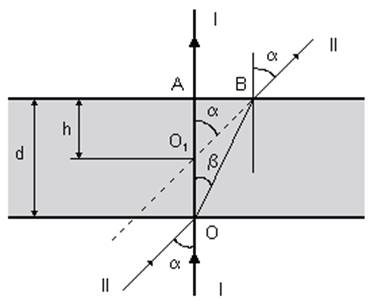
\includegraphics[width=0.6\textwidth]{schemat_zalamanie}
		\end{figure}
	\end{center}

	
	Dla użytego przez nas mikroskopu wartości kątów $\alpha$ i $\beta$ są niewielkie, ponieważ patrzymy na płytkę prawie prostopadle. Dlatego możemy przyjąć następujące zależności:
	\begin{equation}
		\frac{\sin \alpha}{\cos \beta}=\frac{ \alpha}{ \beta}=\frac{\tan \alpha}{\tan \beta}
	\end{equation}
	
		
	\section{Wykonanie ćwiczenia}
	Ćwiczenie wykonano dla dwóch płytek wykonanych z różnych materiałów (pleksiglas i szkło).
	Dla każdej płytki wykonano następujące czynności:
	\begin{itemize}
		\item W pierwszym kroku przy pomocy markera narysowano na płytce trzy krzyżyki w równej odległosci od siebie.
		W ten sposób, aby po jednej stronie przeźroczystej płytki znalazło się jedno ramię krzyżyka.
		\item 
			Przy użyciu śruby mikrometrycznej dokonano pomiaru grubości płtki w 
			środkach każdego krzyżka.
		\item Zamontowano płytki w uchywcie mikroskopu. 
		\item Przy pomocy pokrętła regulowano położenie stolika, tak aby uzyskać ostry obraz 
		górnego ramienia pierwszego krzyżka.  Odczytano pomiar z mikroskopu. Dwukrotnie zmieniono położenie płytki i powtórzono pomiary dla górnego obrazu.
		\item Następnie dokonano trzech pomiarów dla dolnego ramienia pierwszego krzyżyka.
		\item Przesunięto płytkę i dokonano analogicznych pomiarów dla drugiego i trzeciego krzyżyka.
		\item Uzykane wyniki naniesiono do tabeli ().  
	\end{itemize}
	

	\section{Opracowanie danych pomiarowych}\label{sec:opr}
	\subsection{Pomiary i ich niepewności.}
		
	
 
	
	\subsection{Opracowanie danych.}\label{sec:drm}
	\begin{enumerate}[label=\alph*)]
		
		\item Analiza błędów.
		
		
		\item Obliczenie wartości współczynnika załamania dla szkła i pleksiglasu.
	
		
		\item Niepewności wyliczenia współczynnika załamania
		
		
		\item Otrzymano następujące wyniki:
		\begin{center}
			\begin{tabular}{|c|c|c|}
				\hline Rodzaj materiału & $n$ obliczone & $n$ tablicowe \\
				\hline szkło & 1,53 & 1,50–1,54 \\
				\hline szkło akrylowe & 1,50 & 1,49 \\  
				\hline 
			\end{tabular} 
		\end{center}

	
	\end{enumerate}
	
	\section{Podsumowanie}
	\begin{center}
	
	\end{center}
\vspace{1em}


\end{document}